\documentclass{article}
\usepackage[dblblindworkshop]{neurips_2026}
\workshoptitle{Machine Learning and the Physical Sciences (ML4PS)}
\usepackage[utf8]{inputenc}
\usepackage[T1]{fontenc}
\usepackage{amsmath}
\usepackage{booktabs}
\usepackage{graphicx}
\usepackage{microtype}
\usepackage{xcolor}
\usepackage{url}
\usepackage{hyperref}
\newcommand{\method}{JEPA+SIGReg}
\newcommand{\clipmodel}{CLIP}
\setlength{\bibsep}{2pt plus 0.3ex}

\title{Alignment Is Not One Thing:\\
Contrasting Shared Geometry and Pair Retrieval in Galaxy Images and Spectra}
\author{Anonymous Authors}

\begin{document}
\maketitle

\begin{abstract}
Astronomical surveys observe the same galaxy through complementary modalities, making cross-modal representation learning attractive for retrieval and physical inference.
Yet alignment is usually judged by a single metric.
We compare two end-to-end models trained from random initialization on the same 307,428 paired galaxy images and spectra: symmetric contrastive InfoNCE (CLIP) and direct cross-modal invariance regularized by Sketched Isotropic Gaussian Regularization (JEPA+SIGReg).
Although CLIP is 2.7$\times$ better at bidirectional recall@10, JEPA+SIGReg has higher cross-modal linear CKA (0.770 vs.\ 0.634), distance correlation (0.607 vs.\ 0.485), and held-out linear predictability ($R^2=0.749/0.736$ vs.\ $0.551/0.549$).
Frozen probes reveal a complementary asymmetry: JEPA+SIGReg images retain more physical information, whereas CLIP spectra do.
These results separate pair, geometric, and information alignment, and show that stronger instance matching need not imply a more globally shared representation.
\end{abstract}

\section{Introduction}

Galaxy images encode morphology and projected light, while spectra expose redshift, stellar populations, and emission lines.
Their natural pairing offers supervision without manual labels.
AstroCLIP showed that separately pretrained image and spectrum transformers can be aligned into a useful common space \citep{parker2024astroclip}; more broadly, CLIP-style objectives learn correspondences by identifying a positive among in-batch negatives \citep{radford2021clip}.
Joint-embedding predictive architectures instead match views without explicit negatives \citep{assran2023ijepa}.
LeJEPA couples a predictive invariance loss with SIGReg, which regularizes random one-dimensional projections toward an isotropic Gaussian and prevents collapse without a teacher or stop-gradient \citep{balestriero2025lejepa}.

These losses encode different inductive biases, but evaluations often compress alignment to retrieval.
Exact retrieval tests instance discrimination; it does not ask whether two modalities preserve the same global relations, whether one representation is linearly recoverable from the other, or which scientific variables remain accessible.
For galaxies this distinction is especially important: many objects have plausible physical analogues, so a scientifically coherent neighbor may still be an incorrect instance match.

We perform a controlled, sample-matched comparison between contrastive and regularized-invariance training for galaxy images and DESI spectra.
Our contributions are:
(i) a taxonomy and diagnostic suite separating \emph{pair}, \emph{geometric}, and \emph{information} alignment;
(ii) evidence that CLIP improves exact and local matching while JEPA+SIGReg yields a more globally congruent and linearly transformable manifold; and
(iii) an analysis of shared versus modality-private scientific information, including a supporting comparison to frozen-backbone post-training.
The conclusion is not that either loss dominates, but that objective choice selects the kind of alignment obtained.

\section{Models and experimental design}
\label{sec:method}

\subsection{Data and architecture}

We train on 307,428 matched objects assembled from DESI spectra \citep{desi2024edr} and Legacy Survey images \citep{dey2019legacy}.
Each model uses the same randomly initialized ViT-L/14 image encoder, 12-layer 768-dimensional spectrum transformer, modality-specific multilayer projectors, and 256-dimensional objective-facing embeddings.
Both see two augmented image views and two spectrum views for 50 epochs (15.36M object presentations), with all backbone and projector parameters updated.
The models contain approximately 392M parameters.

\paragraph{Regularized invariance.}
For image views $x_i^{(v)}$, spectrum views $x_s^{(u)}$, encoders $f_m$, and projectors $g_m$, let $z_m=g_m(f_m(x_m))$.
The implemented loss is
\begin{equation}
\mathcal L_{\mathrm{J}}
=0.95\,\frac{1}{4}\sum_{v=1}^{2}\sum_{u=1}^{2}
\lVert z_i^{(v)}-z_s^{(u)}\rVert_2^2
+0.05\,\frac{\mathcal R_{\mathrm{SIG}}(z_i)+\mathcal R_{\mathrm{SIG}}(z_s)}{2}.
\label{eq:jepa}
\end{equation}
SIGReg uses 1,024 random slices and 17 evaluation points per slice.
We call this model JEPA+SIGReg for brevity, but stress that it is direct cross-modal invariance, not predictor-based masked I-JEPA: it has no EMA teacher, stop-gradient target, or unimodal loss.

\paragraph{Contrastive alignment.}
The CLIP loss averages symmetric global-batch InfoNCE over the same four image--spectrum view pairings, with $\ell_2$-normalized embeddings and a learned temperature initialized to 0.07.
Both objectives are optimized on four GPUs.
JEPA+SIGReg uses global batch 256 for 60k updates (10.2 hours); CLIP uses global batch 128 for 120k updates (11.1 hours).
Thus sample exposure and wall time are closely matched, while batch size, negatives, and update count remain confounded.

\subsection{Evaluation protocol}

We extract representations for the 168,280-object AstroCLIP benchmark mirror, retaining its 138,583/29,697 historical train/test split.
The 307k unlabeled training union contains identities from this mirror; consequently, probe and mapping heads are held out, but representation evaluation is \emph{transductive}, not an unseen-object benchmark.
Unless stated otherwise, alignment metrics use the 256-dimensional projected embeddings on the 29,697-object test candidate pool.

\emph{Pair alignment} is exact bidirectional retrieval over every candidate, plus cross-modal overlap between exact cosine $k$-nearest-neighbor sets.
\emph{Geometric alignment} uses linear CKA \citep{kornblith2019cka} over all 168,280 rows and Spearman correlation between cosine similarities for 500k deterministic random object pairs.
\emph{Information alignment} fits ridge maps in each direction, selects regularization on a train-only validation carve-out, refits on the remaining training rows, and reports global held-out $R^2$.
Scientific accessibility is evaluated with standardized ridge probes for redshift and four PROVABGS properties \citep{hahn2023provabgs} on 73,341/15,993 train/test objects.
We average three probe seeds; their standard deviations are below $8\times10^{-4}$, so Table~\ref{tab:probes} reports means.

\section{Results}

\subsection{The objectives learn different alignments}
\label{sec:alignment}

\begin{figure}[t]
  \centering
  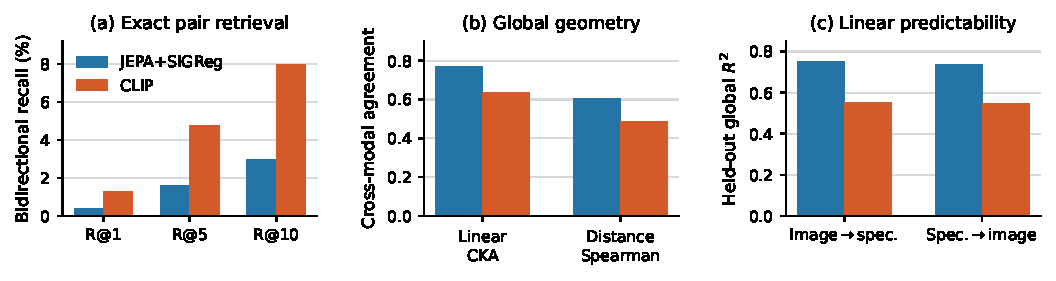
\includegraphics[width=\linewidth]{Figures/alignment_tradeoffs.pdf}
  \caption{\textbf{Alignment is multidimensional.} On the same representations, CLIP is stronger at exact pair retrieval, whereas JEPA+SIGReg better preserves global geometry and supports cross-modal linear prediction. Retrieval is the bidirectional mean on the 29,697-object pool; CKA uses all 168,280 objects.}
  \label{fig:tradeoffs}
\end{figure}

Figure~\ref{fig:tradeoffs} shows a clean reversal.
CLIP reaches bidirectional R@1/5/10 of 1.27/4.76/7.98\%, compared with 0.39/1.62/2.97\% for JEPA+SIGReg.
Its median ranks are also lower: 230 vs.\ 429 for image-to-spectrum and 270 vs.\ 454 in the reverse direction.
Against the harder 168,280-object pool, the ranking persists (mean R@10 2.12\% vs.\ 0.63\%).
Contrastive negatives therefore produce substantially better instance discrimination.

Global structure gives the opposite result.
Cross-modal projected CKA is 0.770 for JEPA+SIGReg and 0.634 for CLIP; pairwise-similarity Spearman correlation is 0.607 and 0.485, respectively.
The raw backbones show the same ordering (CKA 0.898 vs.\ 0.832), so this difference is not only a projector artifact.
Local geometry, however, favors CLIP: test-set cross-modal neighbor overlap at $k=10$ is 2.62\% vs.\ 1.70\% (at $k=100$, 10.97\% vs.\ 10.49\%).
Together, these metrics locate CLIP's advantage at the instance/local scale and JEPA+SIGReg's at the global scale.

The strongest separation is information alignment.
A held-out linear map explains 74.9\% of spectrum-embedding variance from JEPA+SIGReg images and 73.6\% in the reverse direction, versus 55.1\% and 54.9\% for CLIP.
Mean cosine similarity after prediction is likewise 0.840/0.830 vs.\ 0.698/0.679.
An orthogonal Procrustes map only modestly improves retrieval for either model, indicating that the spaces differ by anisotropic scaling, subspace selection, and private variation rather than a simple rotation.

\subsection{Shared alignment and private scientific information}

\begin{table}[t]
\centering
\caption{\textbf{Frozen ridge-probe $R^2$ on raw backbones.} Within each modality, bold marks the better objective. Spectra favor CLIP; images favor JEPA+SIGReg.}
\label{tab:probes}
\small
\setlength{\tabcolsep}{4.2pt}
\begin{tabular}{llccccc}
\toprule
Objective & Modality & Redshift & Mass & Metal. & Age & sSFR \\
\midrule
JEPA+SIGReg & Image    & \textbf{.627} & \textbf{.806} & \textbf{.474} & \textbf{.314} & \textbf{.591} \\
CLIP & Image  & .610 & .793 & .465 & .307 & .580 \\
JEPA+SIGReg & Spectrum & .675 & .842 & .549 & .363 & .639 \\
CLIP & Spectrum & \textbf{.678} & \textbf{.846} & \textbf{.567} & \textbf{.391} & \textbf{.663} \\
\bottomrule
\end{tabular}
\end{table}

Alignment does not erase the distinction between the sensing channels.
Table~\ref{tab:probes} shows a consistent branch-specific trade-off: JEPA+SIGReg images are better for all five tested properties, while CLIP spectra are better for all five.
The largest spectrum differences occur for age (+0.028 $R^2$) and sSFR (+0.023), quantities with diagnostic spectral signatures.
The objective-facing projections are more selective than the raw backbones: for example, JEPA+SIGReg spectrum metallicity falls from 0.549 to 0.448, while CLIP falls from 0.567 to 0.509.
Thus a common embedding is a task-dependent bottleneck, not a sufficient replacement for modality-specific features.

We make this distinction operational by decomposing a target embedding into the prediction from the other modality (\emph{shared}) and its residual (\emph{private}).
For JEPA+SIGReg, the shared component alone recovers nearly all mean linearly accessible performance over the five properties: mean $R^2$ is 0.531 for the predicted spectrum component vs.\ 0.535 for the total, and 0.534 vs.\ 0.531 for images.
The residual remains informative (0.107 and 0.071), especially for spectra.
This is a linear predictability decomposition, not a unique information-theoretic partition; residuals also include nonlinear shared structure and mapping error.

\subsection{Joint training versus frozen post-training}

As supporting evidence, we compare JEPA+SIGReg with a sequential system that begins from independently pretrained image and spectrum encoders, freezes both, and trains 2.23M learned-query pooler parameters under the same objective for 10 epochs.
This is a comparison of two practical regimes, not an initialization-only ablation: the joint model updates 392M parameters for 50 epochs.
Nevertheless, all diagnostics agree.
Joint training improves projected CKA from 0.720 to 0.770, cross-modal $k$NN overlap@100 from 3.81\% to 10.49\%, and mean bidirectional R@10 from 0.87\% to 2.97\%.
Its bidirectional linear-map $R^2$ is 0.749/0.736 rather than 0.598/0.627.
The sequential projections have effective ranks 8.83/8.60 out of 256, compared with 20.19/17.94 jointly, suggesting that small frozen adapters converge to a narrower shared manifold.

The raw joint image backbone retains morphology: on Galaxy10, its frozen linear probe obtains $72.22\pm1.26$\% accuracy and $70.19\pm1.30$\% macro-F1, comparable to the independent image backbone ($71.83\pm0.84$\%, $70.23\pm0.90$\%).
The joint shared projection drops to $44.99\pm0.97$\% accuracy.
Cross-modal training therefore preserves image-private structure in the backbone while deliberately filtering it from the common bottleneck.
This motivates exposing both raw/private and shared outputs in scientific multimodal models.

\section{Discussion}

\paragraph{Why can retrieval and geometry disagree?}
Retrieval is a tail statistic: one highly similar impostor can change rank even when the rest of the geometry is faithful.
Indeed, JEPA+SIGReg has the larger matched-minus-random cosine margin (about 0.75 vs.\ 0.30), yet CLIP ranks the correct partner higher.
Mean random similarity misses the competitive tail that InfoNCE directly optimizes; CKA and distance correlation instead aggregate many relations and favor regularized invariance.
This is scale-dependent geometry, not a metric contradiction, although matched-batch training is needed to isolate the mechanism.

\paragraph{What should a scientific representation expose?}
Exact cross-survey association benefits from CLIP's local discrimination; cross-modal imputation and population comparison benefit from the more transformable JEPA+SIGReg space.
Table~\ref{tab:probes} and the morphology result also show that a common projection discards useful channel-specific content.
A practical model should return $(z_{\mathrm{shared}},z_{\mathrm{private}}^{m})$, or at least expose both projected and raw states.
Its evaluation should mirror that interface: retrieval for correspondence, relational metrics for population geometry, cross-prediction for shared accessibility, and modality-specific probes for retained science.

\section{Limitations and broader impact}

Each objective has one representation-training seed, so deterministic full-pool diagnostics do not measure training-seed variance.
The batch and optimizer-granularity confound prevents attributing every difference solely to the loss.
The transductive evaluation can measure representation quality on the observed catalog but not generalization to unseen objects.
Exact instance retrieval also treats physically valid analogues and duplicates as errors.
A decisive follow-up should use object-disjoint training, matched global batches and updates, multiple seeds, a no-SIGReg collapse control, and fully fine-tuned pretrained initialization.

These representations may reduce labeling requirements and support scalable galaxy search, but they inherit survey selection, calibration, and cross-match biases.
They should not be treated as calibrated physical estimators without task-specific validation.
The work uses public astronomical observations and contains no personal data; its main resource cost is compute (about 10--11 GPU-hours on four GPUs per principal run).

\section{Conclusion}

On matched galaxy image--spectrum training, CLIP improves local matching, while JEPA+SIGReg strengthens global geometry and cross-modal prediction.
Models should report all three alignment axes and expose both shared and modality-private outputs.

\clearpage
\bibliographystyle{plainnat}
\bibliography{references}
\end{document}
